\tikzset{every picture/.style={line width=0.75pt}} %set default line width to 0.75pt        

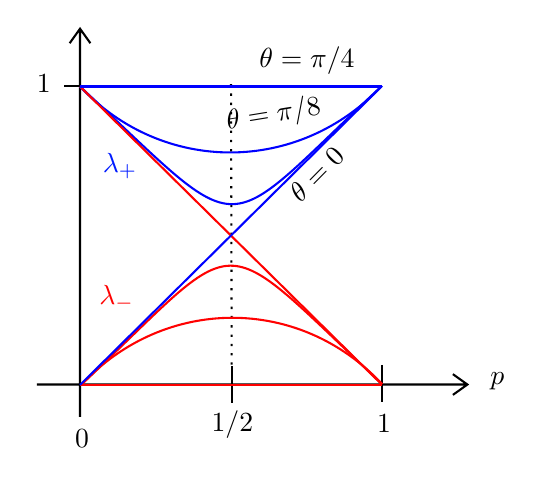
\begin{tikzpicture}[x=0.75pt,y=0.75pt,yscale=-1,xscale=1]
%uncomment if require: \path (0,300); %set diagram left start at 0, and has height of 300

%Shape: Axis 2D [id:dp7922990999691968] 
\draw  (194.43,210.47) -- (401.8,210.47)(215.16,39.04) -- (215.16,226.01) (394.8,205.47) -- (401.8,210.47) -- (394.8,215.47) (210.16,46.04) -- (215.16,39.04) -- (220.16,46.04)  ;
%Straight Lines [id:da8910069240815945] 
\draw    (360.65,200.99) -- (360.65,218.77) ;


%Straight Lines [id:da4351424487889328] 
\draw    (223.72,66.56) -- (207.26,66.56) ;


%Curve Lines [id:da30607876297229386] 
\draw [color={rgb, 255:red, 0; green, 1; blue, 255 }  ,draw opacity=1 ]   (215.16,66.89) .. controls (255,109.31) and (320.33,109.31) .. (360.65,66.55) ;


%Straight Lines [id:da747181608280644] 
\draw    (288.24,201.65) -- (288.24,219.43) ;


%Straight Lines [id:da23659034891816488] 
\draw  [dash pattern={on 0.84pt off 2.51pt}]  (287.91,65.77) -- (288.24,203.63) ;


%Curve Lines [id:da2965920062953322] 
\draw [color={rgb, 255:red, 0; green, 1; blue, 255 }  ,draw opacity=1 ]   (215.16,66.89) .. controls (297.67,143.56) and (280.33,141.46) .. (360.65,66.55) ;


%Straight Lines [id:da39006090585929143] 
\draw [color={rgb, 255:red, 255; green, 1; blue, 0 }  ,draw opacity=1 ]   (215.16,66.89) -- (360.42,210.33) ; %diag. secondaria (rossa)


%Straight Lines [id:da7695278408520292] 
\draw [color={rgb, 255:red, 255; green, 1; blue, 0 }  ,draw opacity=1 ]   (215.16,210.50) -- (360.65,210.50) ;


%Curve Lines [id:da8911454439230475] 
\draw [color={rgb, 255:red, 255; green, 1; blue, 1 }  ,draw opacity=1 ]   (360.76,210.32) .. controls (321.03,167.58) and (255.87,167.58) .. (215.65,210.67) ;


%Curve Lines [id:da5909210917925549] 
\draw [color={rgb, 255:red, 255; green, 1; blue, 1 }  ,draw opacity=1 ]   (360.76,210.32) .. controls (278.47,133.06) and (295.76,135.18) .. (215.65,210.67) ;


%Straight Lines [id:da03926817807025573] 
\draw [color={rgb, 255:red, 0; green, 1; blue, 255 }  ,draw opacity=1 ]   (215.16, 210.67) -- (360.42, 66.89) ; %diag principale (blu)


%Straight Lines [id:da42866181264009473] 
\draw [color={rgb, 255:red, 0; green, 1; blue, 255 }  ,draw opacity=1 ]   (215.16,66.89) -- (360.65,66.89) ;



% Text Node
\draw (416.28,208.92) node   {$p$};
% Text Node
\draw (234.45,105.07) node [color={rgb, 255:red, 0; green, 27; blue, 255 }  ,opacity=1 ]  {$\lambda _{+}$};
% Text Node
\draw (216.16,236.5) node   {$0$};
% Text Node
\draw (361.64,229.26) node   {$1$};
% Text Node
\draw (197.72,65.38) node   {$1$};
% Text Node
\draw (288.57,229.93) node   {$1/2$};
% Text Node
\draw (232.85,168.87) node [color={rgb, 255:red, 255; green, 0; blue, 0 }  ,opacity=1 ]  {$\lambda _{-}$};
% Text Node
\draw (324.5,54.5) node   {$\theta =\pi /4$};
% Text Node
\draw (329,109) node [rotate=-314.59]  {$\theta =0$};
% Text Node
\draw (308.5,80.5) node [rotate=-350.74]  {$\theta =\pi /8$};


\end{tikzpicture}